\documentclass{tufte-handout}

%\geometry{showframe}% for debugging purposes -- displays the margins

\usepackage{amsmath}

% Set up the images/graphics package
\usepackage{graphicx}
\setkeys{Gin}{width=\linewidth,totalheight=\textheight,keepaspectratio}
\graphicspath{{graphics/}}

\title{Developing the Right Near Miss Culture}
\author[CAPT Scott Raymond]{CAPT Scott Raymond, P.E.\newline Executive Officer\newline NAVFAC Europe, Africa, Southwest Asia}
\date{29 Apr 2017}  % if the \date{} command is left out, the current date will be used

% The following package makes prettier tables.  We're all about the bling!
\usepackage{booktabs}

% The units package provides nice, non-stacked fractions and better spacing for units.
\usepackage{units}

% The fancyvrb package lets us customize the formatting of verbatim environments.  We use a slightly smaller font.
\usepackage{fancyvrb}
\fvset{fontsize=\normalsize}

% Small sections of multiple columns
\usepackage{multicol}
\usepackage{multirow}
\usepackage{makecell}
\usepackage{colortbl}
\definecolor{rowcolor}{rgb}{0.92,0.95,0.86}

% Provides paragraphs of dummy text
\usepackage{lipsum}

\usepackage{natbib}
\bibliographystyle{apalike}
\setcitestyle{authoryear}

% These commands are used to pretty-print LaTeX commands
\newcommand{\doccmd}[1]{\texttt{\textbackslash#1}}% command name -- adds backslash automatically
\newcommand{\docopt}[1]{\ensuremath{\langle}\textrm{\textit{#1}}\ensuremath{\rangle}}% optional command argument
\newcommand{\docarg}[1]{\textrm{\textit{#1}}}% (required) command argument
\newenvironment{docspec}{\begin{quote}\noindent}{\end{quote}}% command specification environment
\newcommand{\docenv}[1]{\textsf{#1}}% environment name
\newcommand{\docpkg}[1]{\texttt{#1}}% package name
\newcommand{\doccls}[1]{\texttt{#1}}% document class name
\newcommand{\docclsopt}[1]{\texttt{#1}}% document class option name

\renewcommand\bibsection{
	\section*{Further Reading}
}

\begin{document}
	
	\maketitle% this prints the handout title, author, and date
	
	%\begin{abstract}
	%\noindent 
	%\end{abstract}
	
	%\printclassoptions
	
	This paper addresses near misses (also known as close calls, narrow escapes, near collisions, near hits, and good catches) within Naval Facilities Engineering Command Europe, Africa, Southwest Asia (NAVFAC EURAFSWA).  It provides historical background on "safety pyramids", considers the importance of NAVFAC's near miss culture, identifies the hidden dangers of near misses, and suggests a way forward for improvement.
	
	\section{Significance of Near Misses}\label{sec:SignificanceNearMiss}
	\textsc{Near misses are significant} because they offer an indication of the relative strength of a safety culture.  Reducing near misses also tends to reduce recordable mishaps.  In 1959, Herbert Heinrich published \textit{Industrial accident prevention: a scientific approach} which included the Safety Pyramid shown in Figure~\ref{fig:HeinrichPyramid}.  
	\begin{marginfigure}
		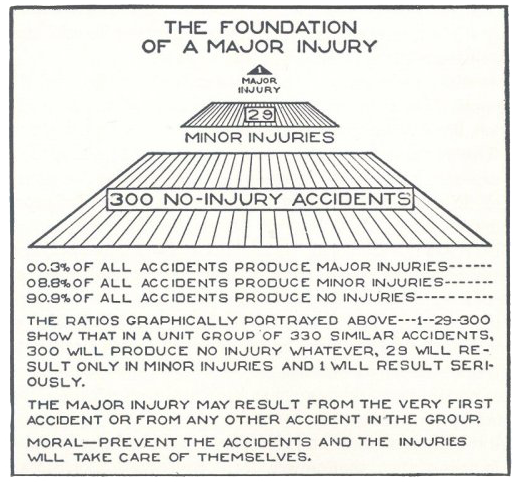
\includegraphics[width=\linewidth]{HeinrichPyramid}
		\caption{Heinrich states the 1:29:300 ratio of major injuries to minor injuries to no-injury accidents he found implies the prevention of no-injury accident (near misses, which account for 88\% of at-risk behavior), will also prevent injuries.}
		\label{fig:HeinrichPyramid}
	\end{marginfigure}
	In 2003, ConocoPhillips Marine conducted a similar study and found near misses represent a far greater ratio than Heinrich believed.  They also added at-risk behaviors to their observations, resulting in a revised Safety Pyramid shown in Figure~\ref{fig:ConocoPyramid}.
	\begin{marginfigure}
		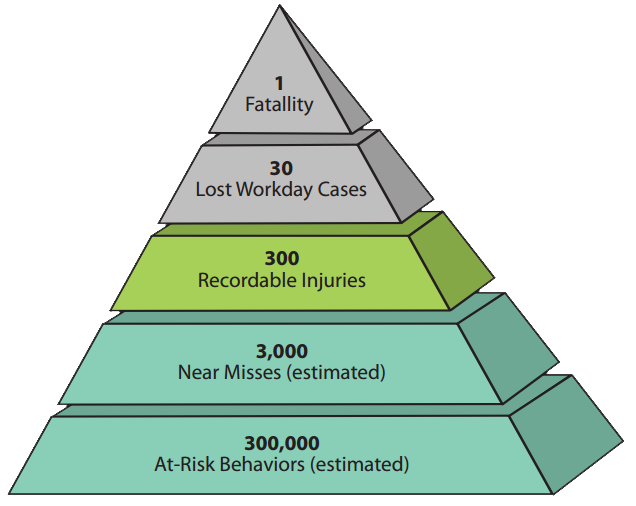
\includegraphics[width=\linewidth]{ConocoPyramid}
		\caption{ConocoPhillips defines "at-risk behaviors" as those activities that are not consistent with safety programs, training and components on machinery.  Together with near misses, they made up 99.9\% of all observable safety misbehavior.}
		\label{fig:ConocoPyramid}
	\end{marginfigure}
	Many safety professionals have suggested the work of Heinrich and others has placed unfounded value on behavior-based safety (BBS), which focuses on employee actions to prevent occupational illness and injury.  However, like the hierarchy of hazard control (which prioritizes elimination, substitution, and engineered controls over administrative controls and PPE) we must not ignore the reduction of mishaps that individual employees can effect, even with system improvements which are certainly more effective.  An analysis of BBS and hazard controls is beyond the scope of this paper.
	
	\newthought{What does NAVFAC's Safety Pyramid} look like?  Unfortunately, given the certain and significant under-reporting of near misses, we don't know.  Regardless, the benefit of near miss reporting remains clear:  it offers an alternative to lagging indicators (usually only mishaps themselves), which even when encouraging are not necessarily conclusive.  In addition to being a leading indicator, near misses also tend to be very localized events, with simple causal analysis that drives straightforward resolution.\marginnote{The absence of a very unlikely mishap is not, in and of itself, an adequate indicator of good safety management - we may be more lucky than good.} 
	
	\section{The Hidden Dangers of Near-Misses}\label{sec:HiddenDangers}
	\textsc{There are hidden dangers of near misses} that result when we interpret the identification and collection of near miss events as evidence that our safety systems are working properly.  
	
	One study \citep{MissedOpportunity} found that participants (students as well as NASA employees and contractors) favorably rated both managers whose decisions resulted in successes as well as those which produced near misses, while adversely rating managers who experienced failures.  This lack of accountability suggests that perception of risk can be lowered after experiencing a near miss.  Such a false sense of system resiliency robs the organization of learning opportunities, which \citeauthor{MissedOpportunity} believe should include the inducement of counterfactual thinking\marginnote{Counterfactual thinking is the psychological process of imagining how an actual event might have turned out given different scenarios of preceding facts.  \textit{Downward} counterfactual thinking considers how the outcome could have been worse - perfect for near miss analysis.}, heightened awareness of how perceptions of risk can change, and making probability	more salient.
	
	Some organizations have embarked on a "Good Catch" program which rebadges the "near miss" label as something good because it was caught before the hazard had sufficient contact time to create a mishap.  By placing a positive spin on the event, it is more likely that employees will report potential errors.  However, this framework leaves a large gap in classification - there is nothing good about some near misses that were never caught in advance of the exposed hazard risking harm, damage, or loss of resources.  Sometimes, we are just lucky to avoid negative consequences - and while that's fortunate, it can't be "good". Unrecognized opportunities for a good catch turn into a near miss, and given enough time, a near miss will turn into a strike.
	
	A focus on simply increasing the number of near miss reports ignores the existence of a gap between expected and actual reporting.  Examining this gap as a blind spot can be uncomfortable and seemingly unproductive when an increase in near miss reports does not lend any insight into controlling the underlying processes that cause the near misses.  Once this gap is eliminated, however, it is then possible to know when actual near miss events are being systematically reduced - and this is the ultimate measure of success in eliminating uncontrolled hazards.
	
	It is a mistake to assume that an increase in near miss reporting, as well as the ultimate reduction in near miss reporting that comes with the elimination of uncontrolled hazards, will reduce mishaps of all severity.  Such a causal relationship would require that the same common causes lead to all types of mishaps.  This is simply not the case.  The common cause of slips, trips, and falls on a congested work site might be poor housekeeping.  But the elimination of housekeeping hazards is unlikely to have any effect on the cause of electrocution.  Conversely, a focus on the prevention of all electrocutions (perhaps a strong commitment to the following of detailed standard operating procedures) will not eliminate housekeeping hazards.
	
	\section{A Better Near Miss Model}\label{sec:BetterModel}
	
	\textsc{It may be more useful to the think of near misses}  \marginnote{Chuck Pettinger, process change leader at Predictive Solutions, offers the following examples:  A \textit{"near hit"} is when a wrench falls from scaffolding and nearly hits a working walking along a designated path.  A \textit{"near miss"} is similar, expect that no one was nearby when the wrench fell.  A site superintendent makes a \textit{"good catch"} when during a routine site walk, she notices wrenches on scaffolding without the required toe boards installed.  If a site safety manager reviews upcoming work tasks and notes a new subcontractor is installing temporary scaffolding, he identifies an \textit{"error likely"} and meets with the team to ensure the plan includes toe boards.} as a continuum for the value of identifying events.  The best situation is when an employee recognizes that an error is likely to occur and becomes involved in the planning process.  These \textit{"error likely"} events drive engagement which requires no reporting and they are evidence that people and processes are effective in proactively supporting the safety culture.  \textit{"Good catches"} are the result of an employee identifying an uncontrolled hazard before someone or something is exposed to harm.  If the good catch goes unrecognized until people or property are in the vicinity of the hazard, it becomes a \textit{"near miss"} and we are fortunate no harm came to be.  When a near miss is so close to a \textit{"near hit"} that we thank luck or divine intervention for lack of a mishap, a significant emotional event provides the most severe opportunity for improvement.
	
	\newthought{NAVFAC, like the rest of the Navy, uses a treatment-based approach} to classify the severity of mishaps.  First aid treatment is the most common and least severe mishap, followed by medical treatment, work restrictions, lost time, and finally, a fatality which is the least common but certainly most severe mishap.  This approach cannot extend to near misses, as there is never an injury to treat if the event is a near miss.  Instead, the use of a hurt-based approach similar to that shown in Table~\ref{tab:SeverityLevels} can be easily adapted to address "potential hurt levels" that could reasonably be the result of a mishap under slightly different circumstances.

	\begin{table*}[ht]
		\centering
		\fontfamily{ppl}\selectfont
		\begin{tabular}{cll}
			\toprule
			Severity Level & Duration & Examples \\
			\midrule
			\rowcolor{rowcolor} \makecell{5\\Multiple Fatalities} & Catastrophe & \\
			%rowdivide
			\makecell{4\\Single Fatality} & Life-Ending & \\
			%rowdivide
			\rowcolor{rowcolor}& & $\bullet$ Amputation/severe disfigurement \\
			\rowcolor{rowcolor}& & $\bullet$ Permanent loss of organ/vision/hearing \\
			\rowcolor{rowcolor}\multirow{-3}{*}{\makecell{3\\Severe Hurt}} & \multirow{-3}{*}{Long-term, Life-Altering} & $\bullet$ Debilitating injuries and illnesses \\
			%rowdivide
			& & $\bullet$ Bone fractures, significant lacerations \\
			& & $\bullet$ Moderate hearing/vision loss \\
			\multirow{-3}{*}{\makecell{2\\Moderate Hurt}} & \multirow{-3}{*}{Weeks to Months} & $\bullet$ Significant lacerations/strains/sprains/burns\\
			%rowdivide
			\rowcolor{rowcolor} & & $\bullet$ Minor lacerations/strains/sprains/burns\\
			\rowcolor{rowcolor} & & $\bullet$ Mild hearing loss/corneal abrasions\\
			\rowcolor{rowcolor} \multirow{-3}{*}{\makecell{1\\Minor Hurt}} & \multirow{-3}{*}{Hours to Days} & $\bullet$ Ergonomic and serious illness events requiring treatment\\
			%rowdivide
			& & $\bullet$ Object in eye removed by flushing\\
			& & $\bullet$ Slips, trips, or falls with no bruising or swelling\\
			\multirow{-3}{*}{\makecell{0\\No Hurt}} & \multirow{-3}{*}{No body damage} & $\bullet$ General soreness\\
			\bottomrule \\
		\end{tabular}
		\caption{Five severity levels adapted from ExxonMobile's Hurt-Based Approach}
		\label{tab:SeverityLevels}
	\end{table*}

	\section{The Way Forward}\label{sec:WayForward}
	\textsc{There are many} best practices for leveraging the value of near miss opportunities.
	\begin{itemize}
		\item Develop a command policy statement\marginnote{Define near miss incidents and clarify their non-recordable but reportable nature.} on near miss reporting which clearly communicates leadership expectations.
		\item Move beyond what to call exposed hazards, and focus on how they are reported and what will be done with them.
		\item Demonstrate the value of near miss reporting by showing employees why their report is able to help someone else in their similar situation and how their report is being used to improve policy and procedure.
		\item Create a climate of non-retribution reporting\marginnote{Reports can first be collected on pre-printed pocket-sized cardstock (quick and easy!) which is then submitted to the Safety Office for entry into ESAMS.} of mishaps and near misses via ESAMS; do not blame employees for their ignorance or shortcuts, but rather re-educate and focus on improvements to the system.
		\item Modify ESAMS to allow for the categorization of reports as good catch, near miss, and near hit.
		\item Implement a hurt-based approach to mishaps and near-misses for both actual and potential severity.
		\item Evaluate risk probability using a quantitative analysis (i.e. 1-in-100 chance) rather than a qualitative analysis (i.e. may occur).
		\item Determine the shape and size of the NAVFAC Safety Pyramid and consider the similarity of mechanisms between severity of mishap.
		\item Highlight the near miss blind spot by comparing expected near miss reports to actual near miss reports.
		\item Implement incentives\marginnote{Gamification - applying the same gameplay mechanisms that attract gamers - represents an innovative incentive strategy.} for the reporting of uncontrolled hazards and near misses; this encourages active observation, participation, and program buy-in.
		\item Set expectations for near miss reporting\marginnote{Better to have 100 employees reporting one near miss each, rather than one employee reporting 100 near misses.} in all Position Descriptions so that  employees understand their responsibility to actively participate.
		\item Model near miss reporting by the most senior employees so that the deckplate sees expected behavior.
		\item Encourage and document good catches,\marginnote{A true good catch is a success event; a near miss is a failure event that causes no harm because of luck.} where people and processes are in place to backstop planning and execution errors before employees and equipment are exposed to uncontrolled hazards. 
		\item Leverage the leading indicator\marginnote{Track trends by classes of near miss across similar units of action and throughout NAVFAC.} nature of near misses to assess the effectiveness of hazard control.
		\item Conduct Mishap Review Boards (MRBs)\marginnote{Most MRBs should be conducted by the chain-of-command, with the oversight of the Safety Office, as soon after the incident as practical.} for all mishaps and near misses that are reasonably preventable or provide opportunity for lessons learned; thorough investigations, even if informal, are essential to understanding the root-cause and other causal factors.
		\item  Assess all safety mishaps,\marginnote{Exxon's "Mining the Diamond" program} including near misses, for both actual and potential consequences by leveraging downward counterfactual thinking (i.e. potential hurt level).
		\item Do not assume a reduction in near misses\marginnote{The mechanisms of near misses are often very different from those of major mishaps.} will result in reduced mishaps; reporting and reducing near misses will improve the safety culture, but uncontrolled critical hazards can harm when least expected.
	\end{itemize}
	
	\nocite{*}
	\bibliography{NearMiss}
	
\end{document}
